\section{Evaluation Practice}
\label{sec:evaluation}

\begin{table*}[t]
\centering
\caption{Responses to degradation by navigation function, the conditions under which they help, and the main evidence gaps, with representative studies.}
\label{tab:synthesis}
\surveytableformat
\begin{tabularx}{\linewidth}{@{}L{2.35cm}YYY@{}}
\toprule
\textbf{Function} & \textbf{Main responses} & \textbf{Conditions for benefit} & \textbf{Main evidence gaps} \\
\midrule
Localization and mapping (Sec.~\ref{sec:localization}) & Selective updates, complementary sensing, motion and contact priors, relocalization, map revision~\cite{P_E01,P_F04,P_E02} & Surviving observable geometry, independent measurements, credible supervision for learned priors, later overlap~\cite{P_S37,P_E07,P_E08} & Mostly recorded or replayed data. Degeneracy and similarity scores differ in meaning. Revised maps rarely drive executed responses~\cite{P_K01,P_R07} \\
\addlinespace[3pt]
Traversability, planning, and control (Sec.~\ref{sec:planning}) & Terrain costs, information-aware exploration, learned prediction, safety filters and risk constraints, delay-aware tracking~\cite{P_K03,P_E13,P_E26} & Accurate pose and terrain coverage, priors and loop opportunities, training coverage, known state and admissible inputs~\cite{P_S45,P_N05,P_M42} & Estimated rather than measured collision risk. Few simulation-to-hardware comparisons. Pose uncertainty rarely propagated into terrain decisions, its effect untested~\cite{P_E25,P_K05} \\
\addlinespace[3pt]
Semantic navigation (Sec.~\ref{sec:semantic}) & Semantic memory, geographic grounding, learned actions, language-derived cost layers, candidate selection with embodiment filters~\cite{P_E44,P_M10,P_R26} & Valid map updates, coverage of prior maps or tours, feasible proposed candidates, a local controller valid during pending inference~\cite{P_S43,P_F05} & Incorrect or stale reasoning rarely injected. GPS, cloud, and map-preparation dependencies. Few physical trials per route~\cite{P_S44,P_S40,P_R25} \\
\addlinespace[3pt]
Multi-robot coordination (Sec.~\ref{sec:multi}) & Allocation and spatial partition, compact sharing, distributed and asynchronous estimation, rendezvous, estimate repair after reconnection~\cite{P_R22,P_R21,P_R19} & Compatible shared inputs, reachable encounters, stable front-end odometry, tracked correlations~\cite{P_E34,P_R20,P_F03} & Mostly ideal or modeled communication. Acceptance of stale or biased content after a partition untested on moving teams~\cite{P_R23,P_K07} \\
\addlinespace[3pt]
Fault tolerance and recovery (Sec.~\ref{sec:reliability}) & Analytic redundancy and tolerant control, integrity and runtime monitoring, executed recovery, resource and service management~\cite{P_E51,P_X07,P_E59,P_R32} & A modeled fault channel with remaining actuation, a monitored event that matches the response, trustworthy state for the recovery maneuver~\cite{P_E52,P_M35} & Injected or simulated faults. Restarted or censored trials. Interruptions and human assistance seldom reported~\cite{P_E55,P_N10,P_N17} \\
\bottomrule
\end{tabularx}
\end{table*}

Since most evidence gaps in Table~\ref{tab:synthesis}, which draws Sections~\ref{sec:localization}--\ref{sec:reliability} together, concern how a result was evaluated rather than whether a mechanism exists, this section compares evaluation practice across the reviewed functions.

Evaluation of autonomy under degradation must relate component outputs to executed behavior. The comparison below follows three axes, namely the level at which performance is measured, the conditions under which degradation is tested, and the event and assumptions behind a risk or diagnostic claim. Fig.~\ref{fig:evaluation} connects the three axes through one time-aligned navigation episode with a degraded interval. Table~\ref{tab:evaluation} counts the coded attributes among the \CoreCount{} technical publications for each reviewed function.

\begin{table}[!ht]
\centering
\caption{Reported evaluation attributes among the \CoreCount{} technical publications. Attributes overlap; context publications are excluded.}
\label{tab:evaluation}
\surveytableformat
\begin{tabularx}{\linewidth}{@{}Yr@{}}
\toprule
\textbf{Attribute} & \textbf{Publications} \\
\midrule
\textit{Measurement level} & \\
Component measures & 160 \\
Task outcomes & 128 \\
\addlinespace[3pt]
\textit{Test conditions} & \\
Degradation testing & 130 \\
\addlinespace[3pt]
\textit{Risk and diagnostic assessment} & \\
Integrity/reliability & 14 \\
\bottomrule
\end{tabularx}
\end{table}


\subsection{Measurement, Test Conditions, and Claim Interpretation}

\emph{Component measures} include trajectory, mapping, segmentation, prediction, and tracking error together with runtime and classification scores, whereas \emph{task outcomes} concern completion, collision, coverage, traversal time, intervention, and service availability. \emph{Degradation evidence} describes an experimental condition rather than a metric, in classes of Section~\ref{sec:methodology} that range from injected faults, outages, or varied terrain against a comparator (D1) to difficult sequences, sites, or crowds selected without manipulation (D2) and incidental conditions (D3). A matched nominal control is a stricter variant of D1, used below as a sensitivity definition. For \emph{risk and diagnostic assessment}, the defined event matters, since classifier recall, nominal false-positive control, protection-level coverage, and undetected hazardous error are not interchangeable, as reliable MCL, conformal anomaly detection, and EKF-SLAM integrity illustrate~\cite{P_M35,P_E54,P_X07}.

\subsection{Evidence Across Navigation Functions}

The counts in Table~\ref{tab:evaluation} describe the selected sample rather than the field, and assessment depth varies as disclosed in the supplementary material. Three patterns are nevertheless large enough to qualify the comparisons of Sections~\ref{sec:localization}--\ref{sec:reliability}. First, evidence for localization and mapping stops at the estimate, since all \LocTechCount{} studies report component measures and \LocNamedCount{} name a degradation condition, whereas only \LocTaskCount{} reports a task outcome. Planning and semantic studies show the opposite profile, with task outcomes in \PlnTaskCount{} of \PlnTechCount{} and \SemTaskCount{} of \SemTechCount{} studies. Second, \DegTaskCount{} publications (\DegTaskShare\%) report a task outcome under a named degradation condition in the same experiment, the combination that ties a degraded condition to executed behavior. The share rises from \LocSameShare\% in localization through \MrcSameShare\% in multi-robot coordination, \RelSameShare\% in fault management, and \SemSameShare\% in semantic navigation to \PlnSameShare\% in planning and control. Of these publications, \DOneSameCount{} rest on a condition injected or varied against a comparator and \PhysSameCount{} on a physical robot. Third, the sample contains only \IntegrityCount{} publications with integrity or failure-risk assessment and \ComputeUnreported{} publications that do not report computation placement.

These shares are statistics of the purposively selected sample that depend on definitions and subsets (Table~\ref{S-tab:sensitivity} in the supplementary material). The headline share falls to \DOneNominalShare\% when the condition must be varied against a nominal level, becomes \AnyUnitShare\% when the two attributes may come from different experiments, and was \DegTaskShareCard\% under the card-level coding of an earlier draft. It is \DepthFullShare\%, \DepthLegacyShare\%, and \DepthTargetedShare\% among full, earlier-extraction, and targeted readings, and \WhlShare\% among target wheeled robots against \NonWhlShare\% among other carriers. The share stays between \StageMinShare\% and \StageMaxShare\% when any one selection stage is removed, at \QuotaShare\% in the quota stages against \NonQuotaShare\% elsewhere, and between \YearMinShare\% and \YearMaxShare\% across year bands. In every stage, depth, and quota subset, localization keeps the lowest or a tied lowest share and planning the highest.

\subsection{Execution and Reference Dependence}

\begin{figure*}[!t]
\centering
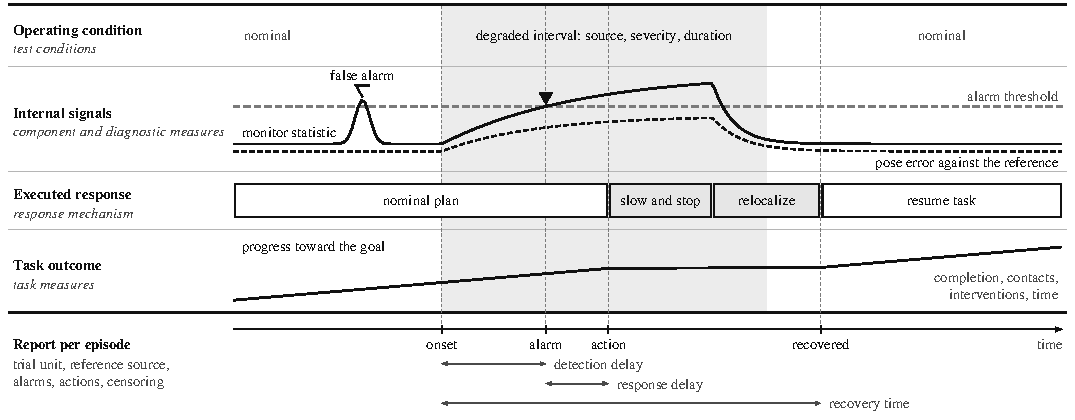
\includegraphics[width=\textwidth]{figures/fig-evaluation.pdf}
\caption{Joint evaluation of detection and response in one navigation episode. The shaded band marks the degraded interval. The operating condition defines the test, internal signals carry component and diagnostic measures, and the executed response and task outcome carry task measures. Detection delay, response delay, and recovery time follow from the synchronized events. A threshold crossing while the pose error stays below the alert limit counts as a false alarm, and an error above the alert limit without a crossing counts as a missed detection.}
\label{fig:evaluation}
\end{figure*}

Recorded measurements preserve sensor artifacts without testing feedback between the estimated state and future observations, whereas closed-loop evaluation lets the evaluated output change the commands and thus the subsequent observations. External pose, offboard processing, teleoperated prior mapping, and staged scenes define the conditions of that feedback, as when slip-aware fusion runs without a controller consuming its estimates~\cite{P_M39} and LiDAR-based barrier control runs under external pose and offboard computation~\cite{P_E26}.

References introduce their own dependence when they share sensors or processing with the evaluated method, as in campus line localization~\cite{P_F01}, kinematic diagnosis with a substitute position~\cite{P_E51}, and orchard map merging scored against its own mapping backbone~\cite{P_S23}. Reference quality also varies within datasets, through the mix of smoothed RTK, offline multisensor SLAM, and selected laser-tracker checks in M2UD~\cite{P_F11}, the untimestamped HK-MEMS bus-route reference~\cite{P_S21}, and scene-dependent reference construction in GEODE~\cite{P_S33}. Cooperative range-only SLAM runs offline on joystick-recorded bags~\cite{P_S27}, whereas hierarchical map transmission reports an estimated risk field from dataset replay rather than measured contacts~\cite{P_R21}. Controlled variables must also match the claimed mechanism. Varying terrain geometry tests plane-fitting allocation~\cite{P_F09}, whereas a test of pose-aware terrain decisions must vary pose uncertainty. Similarly, communication studies rank methods under ideal simulated links in URGE~\cite{P_R22} and replay benchmark factors under modeled connectivity in riMESA~\cite{P_R23}, two settings that do not measure how physical link loss changes the ranking.

\subsection{Guarantees, Rates, and Denominators}

A formal safety result applies to a specified event, probability space, horizon, and set of assumptions. A scenario-planning certificate concerns the risk of an accepted plan under a predicted obstacle distribution~\cite{P_E25}, while environment-level perception calibration depends on representative calibration environments and known state~\cite{P_F08}. A barrier proof may assume feasible inputs for \eqref{eq:cbf} that saturation violates~\cite{P_E26}. Spatiotemporal-tube guarantees likewise assume bounded disturbances and terminal separation without explicit input limits~\cite{P_N12}. None of these guarantees is an empirical closed-loop collision frequency, which must be estimated from executed trials.

Empirical rates require a denominator and an independent trial unit. Across ten homes, the assistive-robot study records 1539 service requests, of which 1130 succeeded, 177 failed, and 232 were not performed~\cite{P_M37}. Its 86.46\% success rate uses the 1307 attempted interventions as denominator and is therefore not the fraction of requests served. Eligibility and censoring change the represented population. Some studies remove scenarios before reporting, as when the CENTAURO study discards infeasible or slowly planned scenarios~\cite{P_N17}. Others remove methods or runs after a failure, as cross-modal teach-and-repeat excludes methods that fail on the first route from later routes~\cite{P_R11}, an outdoor visual-inertial benchmark averages error only over surviving runs~\cite{P_S19}, and multi-session radar mapping omits failed baselines from its averages~\cite{P_R09}. A trial repeated after failed relocalization~\cite{P_N10} differs from recovery within the original attempt. Completion after temporal-logic relaxation~\cite{P_N15} must likewise name the requirements that were changed. Safety and completion must also be reported together, since refusing every action reduces collisions while preventing useful work.

\subsection{Timing, Placement, and Comparisons}

Timing should cover sensing age, transport, perception, estimation, planning, supervision, command delivery, and actuator response, which processor identity and average module runtime do not establish. Fast and slow monitors~\cite{P_F07}, cached reasoning~\cite{P_E60}, slow VLM planning~\cite{P_R26}, and change detection at 2.74\,Hz on an embedded GPU~\cite{P_R07} each need a local controller that stays valid between outputs. DMSA processes data at 1.5--4 times the recording duration and distinguishes unsupported sensor adaptations from failed runs~\cite{P_N20}. Memory-event-triggered MPC counts updates on an industrial computer rather than measuring onboard execution~\cite{P_N14}. A study of LiDAR--inertial non-reproducibility repeats each experiment 30 times after controlling subscribers and buffering~\cite{P_N04}, showing that repeated playback characterizes implementation variability rather than variation across missions.

\begin{table}[!t]
\centering
\caption{Reporting checklist for a joint evaluation of detection and response.}
\label{tab:checklist}
\surveytableformat
\begin{tabularx}{\linewidth}{@{}L{1.9cm}Y@{}}
\toprule
\textbf{Element} & \textbf{What to report} \\
\midrule
Fault model & Source, channel, and channels assumed trustworthy \\
Onset, duration & Onset time, duration, and recovery criterion \\
Severity & Tested levels, including a nominal level \\
Trial unit & Run, route, or mission, with independent repeats \\
Denominator & Attempts, censored or excluded runs, and reasons \\
Reference & Source, coverage, and dependence on tested sensors \\
Alarms & Threshold, alert limit $A_t$ in \eqref{eq:integrity}, false and missed alarms \\
Event times & First alarm at the supervisor and response onset \\
Delay & Detection-to-action delay in each trial \\
Computation & Placement, sensing age, and end-to-end latency \\
Controls & Nominal stack, simple response, and no-fault runs \\
Response & Executed rejection, correction, reset, or maneuver \\
Task outcome & Completion, contact, and interventions, with intervals \\
\bottomrule
\end{tabularx}
\end{table}

\subsection{Joint Evaluation of Detection and Response}

A joint evaluation links degradation onset to an internal trigger, an executed response, and a task outcome within one mission, as Fig.~\ref{fig:evaluation} shows. Table~\ref{tab:checklist} lists what such an evaluation should specify, log, and report, including matched controls that isolate the response mechanism and reveal the cost of unnecessary interventions.
